\documentclass{book}

\usepackage{graphicx}
\graphicspath{ {images/} }

\usepackage[T1]{fontenc}
\usepackage[utf8]{inputenc}
\usepackage{natbib}

% Para símbolos matemáticos
\usepackage{amsfonts} 
\usepackage{amsmath} 

\title{Estudio de viabilidad del uso de librerías de criptografía homomórfica en procesos reales}
\author{Javier Junquera Sánchez}
\date{May 2019}

\begin{document}

\maketitle

\chapter*{Resumen}

\chapter*{Abstract}
\label{chap:abstract}

\chapter*{Agradecimientos}


\tableofcontents{}
% \tableoftables{}
% \tableoffigures{}


% TODO Revisar estructura con plantilla
\chapter{Introducción}
\label{chap:intro}

Para todo $ A,B \in \chi{} $, una operación $ \bigoplus $, y una función $f$; si se cumple $ f(A) \bigoplus f(B) = f(A \bigoplus B)$, $ f $ es una función homomórfica con respecto a $ \bigoplus $ en $ \chi{} $. Cuando una función criptográfica cumple esta condición con alguna operación se dice que es maleable (\cite{dolev_non-malleable_1991}).

Aunque es una propiedad que podría no ser deseable en muchos ámbitos (por ejemplo, en un escenario en el que además de confidencialidad se requiera integridad, permitiría a un atacante modificar los datos), si cumple ciertas condiciones podría tener numerosas aplicaciones. Así se crea el campo de estudio de la criptografía homomórfica.

Se conoce como criptografía homomórfica al conjunto de técnicas criptográficas destinadas a permitir operar con datos cifrados y que dichas operaciones se materialicen correctamente sobre los datos al descifrarlos. En función (principalmente) de las operaciones con las que se cumple esta premisa, o el sistema utilizado para procesar los datos antes y después de operar... Aunque pueda haber muchas variantes de cada una de estas propiedades, la comunidad científica ha establecido criterios y notaciones para su estudio.

\section{Estandarización}

El consorcio "Homomorphic Encryption Standardization" (\cite{albrecht_homomorphic_2018}) ha ido desarrollando un estándar a lo largo de los años atendiendo a los avances en las distintas tecnologías que componen la criptografía homomórfica, y prestando un interés especial en las implementaciones necesarias para ponerla en práctica. Así, se han ido sucediendo las tres generaciones de criptografía homomórfica.

El último encuentro de trabajo del grupo se produjo el 17 de Agosto en Santa Clara, y en él se trabajará principalmente la eficiencia y la usabilidad de las librerías.

La documentación del estándar está dividida en tres \textit{white papers} y una lista de implementaciones conocidas.

\subsection{Seguridad}

En el documento \cite{chase_security_2017} analizan qué principios seguir para implementar esquemas de criptografía homomórfica y qué beneficios tienen estos esquemas para la seguridad de la información. También hacen un análisis de los ataques existentes a estos esquemas y qué parámetros matemáticos son los ideales para hacer estos esquemas lo más resistentes posible tanto en el panorama actual como en un escenario \textit{post-quantum}.

\subsection{Aplicaciones}

En el estudio \cite{archer_applications_2017} abordan para qué campos es útil la criptografía homomórfica. Mientras que se han estado centrando los esfuerzos en poder almacenar información en la nube de forma segura (cifrándola) se ha descuidado la seguridad de dicha información cuando sube a la nube para se procesada. La criptografía homomórfica puede ser la solución a este problema, y en campos como:

\begin{itemize}
    \item La computación distribuida
    \item La protección de datos médicos que tengan que ser procesados en equipos potentes, ajenos a la institución médica
    \item La consulta de información de forma anónima: Por ejemplo, una consulta DNS sin revelar a qué se está accediendo
\end{itemize}

En la última reunión del standard presentaron ejemplos de protocolos de distribución de datos y claves utilizando nuevas implementaciones de esquemas homomórficos (\cite{latigo}).

\subsection{API}

Por último el consorcio de estandarización busca establecer un modelo de almacenamiento común tanto de los datos como de las claves, y una terminología (lo llaman \textit{lenguaje ensamblador}) que sirva de lenguaje común para transmitir las ideas y los elementos mínimos que debe tener cualquier sistema de criptografía homomórfica. Están definidos en el documento \cite{brenner_standard_2017}, y como veremos más adelante, encajan perfectamente con los elementos de las implementaciones. Son los siguientes:

\begin{itemize}
    \item \verb|SecKeygen|, \verb|PubKeygen|

    Tiene que haber un método de generación de clave privada (o secreta) y pública.

    \item \verb|SecEncrypt|, \verb|PubEncrypt|

    Define la posibilidad de que haya además de un sistema de cifrado público (usando la clave pública) que en determinados esquemas se pueda cifrar la información directamente con la clave privada.

    \item \verb|Decrypt|

    Tiene que haber un sistema para restaurar la información desde un texto cifrado.

    \item \verb|Eval|

    La llamada \verb|Eval| será el paraguas que recoja todas las operaciones homomórficas que se puedan realizar sobre el texto cifrado para que luego se materialicen en el descifrado.

\end{itemize}

Algunos esquemas introducirán otras herramientas enfocadas a procesar los datos, pero estarían en niveles superiores de la arquitectura, y son exclusivas de cada implementación.

\section{Objetivo del trabajo}

El objetivo de este trabajo es evaluar si es viable o no utilizar las tecnologías existentes en sistemas y procesos reales. Estudiaremos qué implementaciones hay, en qué consisten, y cuales serán las más idóneas (las más avanzadas, que puedan servir de muestra para inferir la viabilidad de las demás) atendiendo a:

\begin{itemize}
    \item La facilidad de uso: A fin de cuentas la documentación existente y la mayor o menor facilidad de uso se traduce en horas de salario de trabajadores altamente cualificados.
    \item Las capacidades de la tecnología: O qué problemas pueden resolverse con ella
    \item La eficiencia de la solución: Estudiar los tiempos de ejecución de las operaciones
\end{itemize}

\chapter{Estudio teórico}

\section{Tipos}

- Partially homomorphic

- Somewhat

- Leveled fully

- Fully

\section{"Primitivas"}

\subsection{Lattice based encryption}

\subsection{Learn With Errors}

\section{Esquemas por generación}

\subsection{Pre}



\subsection{Primera generación}



\subsection{Segunda generación}

- BGV

https://eprint.iacr.org/2011/277

- BFV

https://eprint.iacr.org/2012/144

\if false
The BFV scheme cannot perform arbitrary computations on encrypted data.
    Instead, each ciphertext has a specific quantity called the `invariant noise
    budget' -- or `noise budget' for short -- measured in bits. The noise budget
    in a freshly encrypted ciphertext (initial noise budget) is determined by
    the encryption parameters. Homomorphic operations consume the noise budget
    at a rate also determined by the encryption parameters. In BFV the two basic
    operations allowed on encrypted data are additions and multiplications, of
    which additions can generally be thought of as being nearly free in terms of
    noise budget consumption compared to multiplications.
\fi

% A paper by Costache and Smart [CS16]gives some initial comparisons between BGV, BFV

- CKKS

No está descrito en el estándar, pero sí se implementa en SEAL.

https://link.springer.com/chapter/10.1007%2F978-3-319-70694-8_15

- TéCnIcA BoOtsTrApPiNg

% https://link.springer.com/chapter/10.1007/978-3-642-30057-8_1

% TODO ¿¿¿¿¿¿¿¿NADIE USA LATTICES???????????

\subsection{Tercera generación}

- GSW

\section{Aplicaciones}


\chapter{Implementaciones}
\label{chap:libs}

\section{Librerías}

Hay varias implementaciones de criptografía homomórfica, y varias soluciones por cada una de las generaciones. Aunque la mayoría de las implementaciones están escritas para \verb|C/C++/C#| Recientemente han ido apareciendo algunas nuevas que buscan, principalmente, adaptar los esquemas de cifrado a otros lenguajes. Aunque esto es una nueva noticia, nosotros nos centraremos en las "clásicas" evaluadas por el consorcio de standarización:

\begin{itemize}
    \item Segunda generación
    \begin{itemize}
        \item HELib
        \item Microsoft SEAL
        \item PALISADE
        \item HeaAn
        \item LoL
        \item NFLlib
    \end{itemize}
    \item Tercera generación
    \begin{itemize}
        \item TFHE
        \item FHEW
        \item cuHE
    \end{itemize}
\end{itemize}

Para nuestro trabajo utilizaremos las librerías Microsoft SEAL (como representante de la segunda generación de criptografía homomórfica) y THFE (como representante de la tercera). Para la segunda generación habría sido también una muy buena opción utilizar PALISADE, pero la documentación es mucho menor, y no incluye el esquema CKKS (necesario para trabajar con números reales).

\section{Microsoft SEAL}
\label{tag:msfseal}

Esta librería de código abierto desarrollada por Microsoft (\textit{SEAL} de ahora en adelante) busca ofrecer una opción asequible para los desarrolladores de implementar soluciones con criptografía homomórfica.

Es muy fácil de instalar, no tiene dependencias externas, y está diseñada para ser construida en cualquier entorno con \verb|cmake|.

Cuenta con dos esquemas de cifrado de segunda generación (BGV y CKKS) y dentro de su código fuente se incluyen varios ejemplos que muestran cómo se opera con ella. En estos ejemplos, ordenados para conocer las distintas herramientas, muestran todo lo necesario para empezar a trabajar.

A la hora de implementar una idea en SEAL, hay dos aspectos clave a tener en cuenta:

\begin{enumerate}
  \item Elegir el esquema de cifrado que nos permita codificar todo correctamente
  \item Estudiar si la operación realmente es realizable con estos esquemas (recordemos que SHE tiene una cota de cómputo)
\end{enumerate}

Además, hay que ser consciente de que bajo determinados usos, puede ser insegura. Por ejemplo, no se debe permitir el descifrado desde un entorno no controlado (no es CCA seguro (\cite{peng_danger_2019})).

\subsection{API}

La API para operar con SEAL está codificada en los siguientes elementos:

\begin{itemize}
  \item EncryptionParameters

  Parámetros descriptivos de los elementos criptográficos

  \item SEALContext

  Contexto del texto cifrado (cambia a medida que se opera)

  \item Claves

  \begin{itemize}

    \item SecretKey

    Clave secreta para descifrar los datos

    \item PublicKey

    Clave pública para descifrar los datos

    \item RelinKeys

    Claves públicas para realinearizar los datos y reducir el nivel de error acumulado tras operar

    \item GaloisKeys

    Claves públicas para trabajar con rotaciones en los vectores cifrados (en nuestro ejemplo no las usamos)

  \end{itemize}

  \item Encryptor, Decryptor

  Sistemas para cifrar y descifrar los datos

  \item Evaluator

  Es el componente que realiza las operaciones sobre los datos cifrados

  \item Encoders

  Encargado de codificar los datos en función del esquema que se desee utilizar

\end{itemize}

A continuación explicaremos más detalladamente el funcionamiento de los componentes más complejos.

\subsection{EncryptionParameters}

Los parámetros criptográficos dependerán del esquema con el que se quiere trabajar.

\begin{itemize}

  \item BFV

  BFV es el esquema "básico" de SEAL. Permite trabajar con números enteros, y operar con ellos hasta que se alcanza el límite máximo de error. En BFV, este límite se podría conceptualizar como un cubo de fichas que se gastan cada vez que se opera.

  Hay algunas operaciones que son casi gratuitas (la suma y la resta), y la multiplicación es muy costosa. Una vez se vacía este cubo (codificado en el parámetro \verb|noise_budget|), nuestro cifrado quedará corrupto y no se puede recuperar el texto.

  Además de \verb|noise_budget|, hay tres parámetros configurables que guardan una estrecha relación:

  - \verb|poly_modulus_degree|

  Determina el módulo del polinomio usado para realizar las operaciones criptográficas (recordemos que implementa LWE sobre un anillo de polinomios, ver \ref{tag:bfv}). Se expresará como una potencia de 2 que cuanto más grande sea, más operaciones permitirá hacer, pero serán más lentas.

  - \verb|coeff_modulus|

  Es un vector de números primos que determina el módulo del texto cifrado. A mayor módulo, mayor será el \verb|noise_budget|. Cuando decíamos que a mayor \verb|poly_modulus_degree|, podíamos hacer más operaciones, era porque el número de bits de \verb|coeff_modulus| está acotado por el de \verb|poly_modulus_degree| de la forma indicada en la figura \ref{table:poly_vs_coeff_modulus}

    \begin{table}
        \centering
        \begin{subtable}
            \centering
            \begin{tabular}{  c  c  }
                \hline
                \verb|poly_modulus_degree|  & Número de bits de \verb|coeff_modulus| \\ [0.5ex]
                \hline
                \hline
                1024  & 27  \\
                2048  & 54  \\
                4096  & 109 \\
                8192  & 218 \\
                16384 & 438 \\
                32768 & 881 \\ [1ex]
                \hline
            \end{tabular}
      \end{subtable}
       \caption{Relación entre \textit{poly\_modulus\_degree} y y el número de bits de \textit{coeff\_modulus\_degree}}\label{table:poly_vs_coeff_modulus}

    \end{table}

  - \verb|plain_modulus|

  Modulo del texto plano. El consumo de \verb|noise_budget| se produce de forma logarítmica en base al tamaño de \verb|plain_modulus|, por lo que cuanto más pequeño es, más operaciones podremos realizar. También debe ser menor que \verb|poly_modulus_degree|.

  \item CKKS

  En la implementación del esquema CKKS podremos trabajar con número decimales, pero tendremos que realizar algunas gestiones adicionales a las de BGV para evitar que se pierda la integridad de nuestros cálculos.

  Comparte con BGV tanto \verb|poly_modulus_degree| como \verb|coeff_modulus|, pero desaparece el elemento \verb|plain_modulus| (la integridad del texto cifrado ya no se evaluará con el \verb|noise_budget|), y los valores elegidos para \verb|coeff_modulus| tendrán otras implicaciones.

  Aparece un elemento nuevo: la escala. De forma análoga a la que hemos implementado en la maqueta de THFE (ya lo veremos en \ref{chap:poc}) para codificar los números decimales se aplica una escala (se multiplican por un valor muy alto, potencia de 2) y se tratan como número enteros.

  Esta escala aumentará drásticamente cada vez que se multipliquen dos elementos. Siendo $N$ el tamaño del primer factor, y $M$ el del segundo, el resultado del producto tendrá como tamaño $M+N-1$. Para evitar que el número desborde su tamaño máximo, tras un producto puede reducirse la escala. La operación de reescalado implementada en SEAL trunca el valor del texto cifrado tantos bits como tenga el último elemento del vector \verb|coeff_modulus|, y elimina este elemento (cambiando el contexto de cifrado). De esta forma, siendo $P$ el tamaño del elemento eliminado de \verb|coeff_modulus| el texto cifrado pasaría a tener un tamaño $(M+N-1)/P$. Una vez se terminan los elementos de \verb|coeff_modulus| no se puede seguir operando, y se debe conservar siempre uno para poder realizar la operación de descifrado.

  Para poder reescalar sin problemas se debe elegir una escala inicial menor que el número expresado por el último valor de \verb|coeff_modulus| (cuando \verb|coeff_modulus| está integro). Además, el primer valor de la cadena (el que se utilizará cuando se vaya a descifrar), debe ser mayor que el resto para poder tener cierta precisión: si este valor es 60, y el segundo (el que se utiliza al realizar la última operación) es 40, tendremos 20 bits de precisión ($60 - 40$) para los decimales al retirar la escala.

  A continuación veremos en qué consiste exactamente el contexto.

\end{itemize}

\subsection{SEALContext, niveles de error y realinearización}

\verb|SEALContext| (lo que llamamos contexto, o contexto criptográfico) es la clase en la que se codifican las propiedades del texto cifrado, desde el esquema utilizado a los distintos parámetros de cifrado. La creación del \verb|SEALContext| genera una estructura similar a una cadena que guardará el estado de \verb|coeff_modulus|. De esta forma, podremos mantener la integridad al operar entre distintos textos cifrados símplemente verificando que esta cadena es igual.

Inicialmente, la cadena se inicializa con la información de \verb|coeff_modulus|, y va cambiando a medida que, por ejemplo, se aplican operaciones de reescalado. La cadena es una lista enlazada de los \verb|SEALContext| en cada momento de operación:

\begin{listing}[ht]
    \begin{minted}{console}
         special prime +---------+
                                 |
                                 v
coeff_modulus: { 50, 30, 30, 50, 50 }  +---+  Level 4
                                          |
                                          |
   coeff_modulus: { 50, 30, 30, 50 }  +---+  Level 3
                                          |
                                          |
       coeff_modulus: { 50, 30, 30 }  +---+  Level 2
                                          |
                                          |
           coeff_modulus: { 50, 30 }  +---+  Level 1
                                          |
                                          |
               coeff_modulus: { 50 }  +---+  Level 0
    \end{minted}
    \caption{Cadena de SEALContext (documentación de SEAL)}\label{fig:seal_levels}
\end{listing}

Se puede descender, pero nunca ascender. Cuanto más abajo, más rápidos son los cálculos, pero menos cálculos se pueden hacer. En ocasiones, debido al tamaño del texto plano, descender no tendrá consecuencias en cuanto al nivel de error, por lo que se podrá hacer para tener mayor eficiencia. En otros, será una condición indispensable para poder seguir operando. Es por esto que, cumpliendo los requisitos sobre el tamaño de \verb|coeff_modulus| con respecto a \verb|poly_modulus_degree|, y siguiendo las pautas que hemos comentado con respecto al primer y último elemento de la cadena, elijamos el mayor número de elementos intermedios posible.

Mientras que en BGV este contexto no tiene mucha importancia (más allá de la eficiencia) en CKKS la cosa cambia. Cuando se reescala en CKKS, se está eliminando al mismo tiempo parte de esta cadena. Por lo tanto, hay que tener en cuenta que si se ha reescalado, y se ha cambiado el contexto de cifrado de un elemento, tendremos que ajustar el contexto del resto de elementos que queramos operar con él (para que estén en la misma escala y usen los mismos parámetros criptográficos), ya sea reescalando (cuando sea necesario) o haciendo al elemento "descender" en la cadena.

Otra forma de reducir la velocidad a la que aumenta el nivel de error sin perder profundidad computacional (capacidad para realizar más operaciones) es la realinearización. Como hemos visto anteriormente, a medida que se opera, el error aumenta. La suma es casi gratuita, pero con el producto de dos elementos de tamaño $M$ y $N$, teniendo el resultado tamaño $M+N-1$, el error aumenta considerablemente. Interpretaremos este tamaño como el grado polinómico del elemento. La realinearización es una operación que permite, utilizando unas claves especiales (claves de realinearización), reducir el tamaño tras una multiplicación, reduciendo así el consumo de \verb|noise_budget| en las siguientes operaciones. Tiene un coste computacional alto en comparación con el resto de operaciones, pero permite operar de forma más eficiente, y que el elemento no crezca hasta "romperse" (o crezca de una forma más lenta).

\subsection{Encoders}

SEAL ofrece tres sistemas para codificar los datos con los que se va a trabajar:
\begin{itemize}
    \item \verb|IntegerEncoder| (para BFV)

    Codifica el número descomponiendolo en una sucesión de exponenciaciones para poder trabajar con sus subelementos de forma independiente.

    \item \verb|BatchEncoder| (para BFV)

    Crea una matriz $2x(N/2)$ con N el número de elementos codificables. Estos elementos son conocidos como \textit{slots}, y su número es igual a \verb|poly_modulus_degree|. En cada \textit{slot} se almacena un número módulo \verb|plain_modulus|. Si se codifica un vector, se introducirá tal cual, y si sólo se codifica un valor, se llenarán todas las posiciones de la matriz con ese valor.

    \begin{gather}
      a =
      \begin{pmatrix}
        a & a & \hdots & a \\
        a & a & \hdots & a
      \end{pmatrix} &
      \begin{pmatrix}
        c_1 & c_2 & c_3
      \end{pmatrix}
      =
      \begin{pmatrix}
        c_1 & c_2   & c_3   & 0     & \hdots & 0 \\
        0   & 0     & 0     & 0     & \hdots & 0
      \end{pmatrix}
    \end{gather}

    \item \verb|CCKSEncoder|

    Funciona de forma similar al \verb|BatchEncoder|, pero tiene la mitad de posiciones con respecto al mismo \verb|poly_modulus_degree|.
\end{itemize}{}

\subsection{Trabajo con vectores}

Tanto \verb|BatchEncoder| como \verb|CKKSEncoder|, interpretan todos los datos como vectores. Una de las cosas más interesantes de esta forma de codificar los datos, es que se pueden rotar las columnas y las filas. La rotación es cíclica, es decir, cuando se rota una posición a la izquierda el primer valor pasa a la última posición.

\begin{itemize}
    \item Rotando filas
    
    \begin{gather}
        \begin{bmatrix}
            b_{11}  & b_{12}  & \hdots    & b_{1n} \\
            b_{21}  & b_{22}  & \hdots    & b_{2n}
        \end{bmatrix}
        \rightarrow
        \begin{bmatrix}
            b_{12}  & \hdots    & b_{1n}    & b_{11} \\
            b_{22}  & \hdots    & b_{2n}    & b_{21}
        \end{bmatrix}
    \end{gather}
    
    \item Rotando columnas 
    
    \begin{gather}
        \begin{bmatrix}
            b_{11}  & b_{12}  & \hdots    & b_{1n} \\
            b_{21}  & b_{22}  & \hdots    & b_{2n}
        \end{bmatrix}
        \rightarrow
        \begin{bmatrix}
            b_{21}  & b_{22}  & \hdots    & b_{2n} \\
            b_{11}  & b_{12}  & \hdots    & b_{1n} 
        \end{bmatrix}
    \end{gather}
    
\end{itemize}
%
%     [  0,  1,  2,  3,  0, ...,  0,  0,  0,  0,  0 ]
%     [  4,  5,  6,  7,  0, ...,  0,  0,  0,  0,  0 ]
%
% Line  60 --> Encode and encrypt.
%     + Noise budget in fresh encryption: 134 bits
%
% Line  78 --> Rotate rows 3 steps left.
%     + Noise budget after rotation: 134 bits
%     + Decrypt and decode ...... Correct.
%
%     [  3,  0,  0,  0,  0, ...,  0,  0,  0,  1,  2 ]
%
%     [  7,  0,  0,  0,  0, ...,  0,  0,  4,  5,  6 ]
%
% Line  92 --> Rotate columns.
%     + Noise budget after rotation: 134 bits
%     + Decrypt and decode ...... Correct.
%
%     [  7,  0,  0,  0,  0, ...,  0,  0,  4,  5,  6 ]
%     [  3,  0,  0,  0,  0, ...,  0,  0,  0,  1,  2 ]

Por otro lado, las operaciones aritméticas se realizan entre los valores de cada posición uno a uno, no como una operación entre matrices. Por ejemplo, el producto sería:

\begin{gather}
    \begin{bmatrix}
        a_{11}  & \hdots    & a_{1n} \\
        a_{21}  & \hdots    & a_{2n}
    \end{bmatrix}
    *
    \begin{bmatrix}
        b_{11}  & \hdots    & b_{1n} \\
        b_{21}  & \hdots    & b_{2n}
    \end{bmatrix} 
    =
    \begin{bmatrix}
        (a_{11} * b_{11})    & \hdots    & (a_{1n} * b_{1n}) \\
        (a_{21} * b_{21})    & \hdots    & (a_{2n} * b_{2n})
    \end{bmatrix}
\end{gather}



\subsection{Evaluator}

Por último, conociendo todo lo que se puede hacer con SEAL, veremos cómo hacerlo. Para trabajar con los elementos cifrados SEAL ofrece las siguientes operaciones, codificadas en la clase \verb|Evaluator|:

\begin{itemize}
    \item negate
    
    Negar (equivalente a multiplicar por $-1$) la variable introducida.
    
    \item add
    
    Función de suma
    
    \item sub
    
    Función de resta
    
    \item multiply
    
    Función de multiplicación
    
    \item square
    
    Función para elevar al cuadrado.
    
    \item exponentiate
    
    Función de exponenciación.
    
    \item rotate
    
    
    
    \item realinearize
    
    
    
    \item mod\_switch
    
    
    
\end{itemize}

Todas las operaciones aritméticas se pueden aplicar para operar tanto entre elementos cifrados como con números en texto plano (símplementecodificados).

\section{TFHE}

En TFHE se trabaja directamente con puertas lógicas. No hay ningún parámetro adicional que seleccionar (mas allá de los relacionados con generar una clave aleatoria), tiene una API simple pero muy potente, pero para hacer cualquier cálculo hay que implementarlo desde el nivel más bajo. Cuando se cifra un dato se genera un array de bits correspondiente al dato cifrado. Será este array (codificado en la clase \verb|LweSample|) sobre el que aplicaremos los algoritmos y procedimientos que diseñaremos, como si trabajásemos con el texto plano.

Los elementos que forman TFHE son mucho menos complejos que los de SEAL, con un único sistema de cifrado (http://lab.algonics.net/slides_ac16/index-asiacrypt.html).

CONTAR: Sólo definir el parámetro $\lambda$ (ver http://lab.algonics.net/slides_ac16/index-asiacrypt.html#/7)

Están codificados en sólo unos pocos grupos:

\begin{itemize}
  \item Parámetros de cifrado (\texttt{TFheGateBootstrappingParameterSet})
  \item Claves: Privada ( (\texttt{TFheGateBootstrappingSecretKeySet})) y pública (\texttt{TFheGateBootstrappingCloudKeySet})
  \item Operaciones de cifrado y descifrado
  \item Operaciones lógicas sobre texto cifrado (\texttt{LweSample})
\end{itemize}

Además, TFHE ofrece funciones para limpiar la memoria, dejando en manos del desarrollador la posibilidad de evitar fugas de información una vez no se va a utilizar un elemento.

\subsection{API}

A continuación haremos un repaso de las principales operaciones sobre el texto cifrado incluidas en la librería TFHE.

\begin{itemize}

  \item bootsCONSTANT

  Carga una constante en \verb|value| en la variable cifrada \verb|result|.

  \begin{lstlisting}[language=c++]
    void bootsCONSTANT(LweSample* result, int value,
                      const TFheGateBootstrappingCloudKeySet* bk);
  \end{lstlisting}

  \item bootsNOT

  Niega el valor de la variable \verb|ca| y lo almacena en \verb|result|.

  \begin{lstlisting}[language=c++]
    void bootsNOT(LweSample* result, const LweSample* ca,
                  const TFheGateBootstrappingCloudKeySet* bk);
  \end{lstlisting}

  % TODO Alinear y verbatim
  % TODO Etiquetar los códigos
  \item bootsCOPY

  Copia el valor de la variable \verb|ca| y lo almacena en \verb|result|. Cuando se utilizan tanto esta función como las funciones \verb|bootsCONSTANT|  y \verb|bootsNOT| se suele trabajar bit a bit iterando sobre los dos arrays. Si no se hace así, a veces pueden tener comportamientos erráticos.

  \begin{lstlisting}[language=c++]
    bootsCOPY(LweSample* result, const LweSample* ca,
              const TFheGateBootstrappingCloudKeySet* bk);
  \end{lstlisting}

  \item bootsMUX

  Es una implementación del operador ternario (\verb|a ? b : c|) esencial para poder introducir cómputos con divergencias en su flujo de ejecución aunque (como hemos comentado anteriormente) no podamos modificarlo. Asigna a \verb|result| el valor de \verb|b| si se cumple \verb|a|, si no, le asigna el valor de \verb|c|.

  \begin{lstlisting}[language=c++]
    bootsMUX(LweSample* result, const LweSample* a,
            const LweSample* b, const LweSample* c,
            const TFheGateBootstrappingCloudKeySet* bk);
  \end{lstlisting}

  Esta función es especialmente interesante, y es la que le da todo el valor a la librería para hacer implementaciones complejas. Por ejemplo, una función con el siguiente código:

  \begin{lstlisting}[language=c++]
    while (result < 100)
      result = result * 2;
  \end{lstlisting}

  No podría ser implementada sin evaluar el valor de result. Sin embargo, con el operador \verb|MUX| podemos hacer lo siguiente (es pseudocódigo):

  \begin{lstlisting}[language=c++]
    /*
     Hasta que el menor valor que podamos
     escribir con los bits que hemos asignado a
     los decimales (10 bits) no sea mayor que 100
    */
    for (int i = 0.001; i < 100; i = i*2) {
      // es_mayor =  result >= 100
      gte(es_mayor, result, 100);
      // factor = es_mayor ? 2 : 1
      bootsMUX(factor, es_mayor, 2, 1);
      // result = result * factor
      multiplica(result, result, factor);
    }
  \end{lstlisting}

  \item Puertas lógicas

  También implementa las siguientes puertas lógicas booleanas. La utilizaremos como base para hacer el resto de operaciones, como por ejemplo la suma (la función de suma es igual que un circuito sumador).

  \begin{itemize}
    \item NAND

    \item OR

    \item AND

    \item XOR

    \item XNOR

    \item NOR

    \item ANDNY, ANDYN

    \item ORNY, ORYN

  \end{itemize}

\end{itemize}

\subsection{Evolución de TFHE}

En su desarrollo se plantea la implementación de un modo conocido como Chimera (\cite{boura_chimera:_2018}) en el que se puedan mover los datos entre el esquema de TFHE y esquemas más eficientes como BFV, CKKS; y viceversa, sin tener que descifrarlos. Por ejemplo, esto puede ser útil para trabajar con muchas puertas lógicas y hacer alguna operación aritmética rápida entre medias.

\chapter{Solución propuesta}
\label{chap:poc}

Como hemos comentado utilizaremos una librería de la segunda generación de criptografía homomórfica (Microsoft SEAL) y otra para la tercera (TFHE). Comenzaremos con un estudio del funcionamiento de las librerías, de cuales son sus límites computacionales y finalmente implementaremos una operación "no trivial" que requiera la utilización de ambas tecnologías.

La librería SEAL cuenta con pocas operaciones aritméticas implementadas, pero ofrece la posibilidad de trabajar con matrices y números decimales. La principal complicación con SEAL es determinar cómo se está desviando el cálculo para saber cuándo parar o qué correcciones hacer. Además, el número de operaciones que puede hacer son muy limitadas (cuando se hacen, por ejemplo productos, crece mucho el error). Por último hay que tener en cuenta que el algoritmo que se implemente en SEAL no puede contener más que sumas, restas y multiplicaciones (no existe la división).

La librería TFHE ofrece una API de operaciones lógicas a nivel de bit. Aunque permitirá hacer cálculos más complejos sin añadir error al resultado, tendremos que implementar todas las operaciones a bajo nivel mediante puertas lógicas, siempre teniendo en cuenta que en ningún momento vamos a poder controlar el flujo de ejecución y nuestros algoritmos tienen que ser capaces de realizar los cálculos sin poder evaluar las variables (están cifradas).

Por lo tanto tenemos que encontrar un cálculo que sea realizable con pocas operaciones y números bajos para SEAL; y operaciones que sean implementables en un tiempo razonable con puertas lógicas para poder trabajar en TFHE.

Se han elegido tanto el sistema de ejemplo como las tecnologías específicas para cada uno de los actores en función de las capacidades y limitaciones de cada tecnología. Como resultado del proyecto se ha creado, además del análisis y el propio código del proyecto, una librería de operaciones matemáticas implementadas en TFHE (\cite{junquera_tfhe_2019}) con puertas lógicas, que es innovadora en tanto en cuanto no existe ningún código público que permita trabajar con TFHE a este nivel.

\section{Funcionamiento del sistema}

Para analizar las librerías implementaremos un sistema de posicionamiento anónimo en función de la temperatura y el mes del año. La base para determinar la posición serán dos curvas de regresión cuadrática de temperaturas de dos ciudades (generada con TFHE), que permitirá que un usuario suba a SEAL la fecha y la temperatura cifradas y averigüe su localización.

En este sistema habrá tres actores: el cliente, el servidor de posicionamiento (programado con SEAL) y un tercer servidor (programado con TFHE) que generará el modelo para calcular la posición. El cliente consultará su posición con el servidor de SEAL, que previamente habrá generado en el servidor de TFHE un modelo de posicionamiento basado en las temperaturas del último año en varias ubicaciones (ver \ref{fig:sistema_completo}).

Generaremos dicho modelo (la curva de regresión $f(x)$) con TFHE porque para ello necesitaremos realizar operaciones aritméticas que no nos ofrece SEAL. De esta forma, podremos realizar la evaluación de los datos introducidos por el usuario con SEAL (distancia entre el valor de temperatura $y$ especificado por el usuario, y $f(x)$ con $x$ el mes del año) utilizando sus operaciones más básicas, y aprovechando su sistema de vectores para evaluar todas las curvas al mismo tiempo.

\begin{figure}[h]
    \centering
    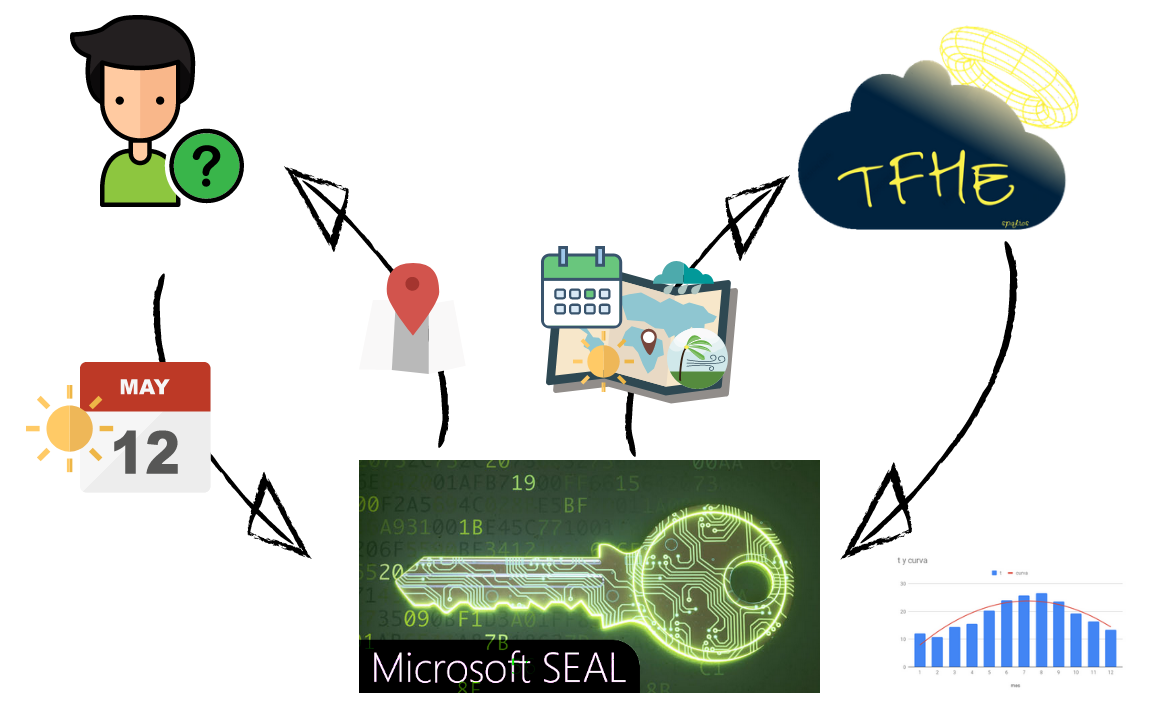
\includegraphics[width=\linewidth]{sistema_completo}
    \caption{Flujo de los datos cifrados (Diagrama generado con Piktochart \url{https://piktochart.com})}
    \label{fig:sistema_completo}
\end{figure}

\subsection{Generación del modelo}

Para generar el modelo el cliente (en este caso, el servidor de posicionamiento con SEAL) y el servidor (el servidor con TFHE) seguirían el siguiente procedimiento:

\begin{enumerate}
    \item El cliente genera un par de claves (pública y privada).

    \item Cifra $n$ pares de datos (en nuestro ejemplo el par sería $(mes, temperatura)$).

    \item Sube los datos cifrados y su clave pública. El número de datos que se puede subir está limitado por el crecimiento del tamaño (en bits) de dichos datos al exponenciarlos para calcular la curva de regresión. Trabajaremos con los datos de 12 meses porque, como comentaremos más adelante\ref{chap:resultados}, aunque el orden máximo al que llegaríamos con estos datos es de 46 bits tendremos otras limitaciones a la hora de procesar los datos.

    \item El servidor procesa los datos y devuelve cifrados los parámetros de la curva

    \item El cliente los descifra y los almacena asociados a una posición geográfica
\end{enumerate}

Finalmente, con los parámetros recibidos, el cliente obtendría una curva similar a \ref{fig:reg2_cg}.

\begin{figure}[h]
    \centering
    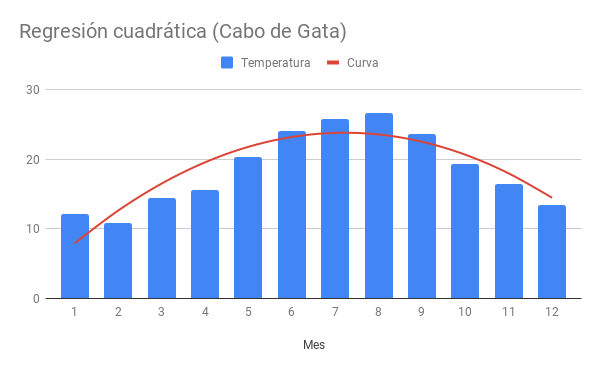
\includegraphics[width=\linewidth]{reg2_cg}
    \caption{Curva de Regresión Cuadrática con temperaturas de Cabo de Gata}
    \label{fig:reg2_cg}
\end{figure}

\subsection{Obtención de la posición}

Teniendo el servidor de SEAL ya generados los modelos de la temperatura de cada ubicación (en este caso, sólo los 2 de Cabo de Gata y Finisterre) el cliente (ahora ya sí, el usuario final) consultará su ubicación:

\begin{enumerate}

  \item El cliente genera tres claves: pública, privada y clave de realinearización.

  \item El cliente cifra (con su clave pública) la temperatura y el mes del año para el que quiere hacer la consulta, generando los valores $y$ e $x$ respectivamente.

  \item Sube ambos valores al servidor, junto con la clave de realinearización (en nuestro ejemplo, no se necesitará subir la pública).

  \item El servidor calculará la diferencia (resta) entre el punto $y$ y $f(x)$ para cada curva

  \item El servidor devuelve una lista con los valores calculados y la ubicación a la que corresponde cada valor

  \item El cliente descifra los valores con su clave privada, obteniendo la distancia entre la temperatura introducida y el valor de la curva de cada una de las ubicaciones ese mes.

\end{enumerate}

En la figura \ref{fig:t_vs_r2} se puede ver un ejemplo del funcionamiento del sistema de posicionamiento. Los puntos introducidos corresponden a las temperaturas de varias ubicaciones, y el sistema de posicionamiento devolvería la distancia entre estos puntos y las dos curvas de regresión. De esta forma se puede obtener una estimación de la posición. En el ejemplo vemos que, la temperatura en Cabo de Gata está muy próxima a su curva en el mes de junio, y daría un resultado indeterminado en abril; que la temperatura de Madrid no casaría con ninguna de las dos curvas; o que la temperatura de Finisterre en noviembre efectivamente está mucho más cerca de la curva de Finisterre que de la de Cabo de Gata.

\begin{figure}[h]
    \centering
    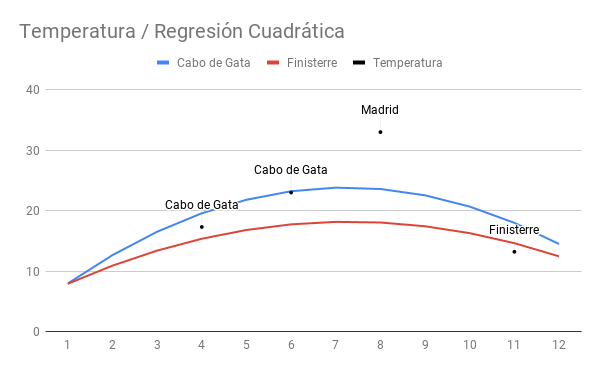
\includegraphics[width=\linewidth]{t_vs_r2}
    \caption{Temperatura vs Regresión}
    \label{fig:t_vs_r2}
\end{figure}

\section{Implementación con TFHE}

Para generar la curva de regresión que utilizará el servidor de SEAL para ubicar al usuario, dicho servidor cifrará los datos de temperatura del último año en dos ubicaciones distintas y se las enviará al servidor TFHE. Este procesa los datos cifrados y calcula la regresión cuadrática codificada en tres parámetros $a, b, c$ que devolverá cifrados al servidor de SEAL.

\subsection{Curva de regresión}

Esta curva $ y = f(x) $ está definida por tres parámetros ($a$, $b$ y $c$) de forma que:

\[ y = ax^2 + bx + c \]

Resultante de resolver el siguiente sistema de ecuaciones:

\begin{gather*}
    \begin{cases}
        \sum_{i=0}^n y_i = a*\sum_{i=0}^n x_i^2 + b*\sum_{i=0}^n x_i + n*c \\
        \sum_{i=0}^n x_i * y_i = a*\sum_{i=0}^n x_i^3 + b*\sum_{i=0}^n x_i^2 + c*\sum_{i=0}^n x_i \\
        \sum_{i=0}^n x_i^2 * y_i = a*\sum_{i=0}^n x_i^4 + b*\sum_{i=0}^n x_i^3 + c*\sum_{i=0}^n x_i^2
    \end{cases}
\end{gather*}

Realizando las siguientes sustituciones:

\begin{align*}
    i &= \sum_{i=0}^n x_i & j &= \sum_{i=0}^n x_i^2 & k &= \sum_{i=0}^n x_i^3 & l &= \sum_{i=0}^n x_i^4 \\
    u &= \sum_{i=0}^n y_i & v &= \sum_{i=0}^n x_i * y_i & w &= \sum_{i=0}^n x_i^2 * y_i
\end{align*}

Obtendríamos un sistema lineal de ecuaciones solucionable mediante eliminación Gauss-Jordan:

\begin{gather*}
    \begin{cases}
        u = a*j + b*i + n*c \\
        v = a*k + b*j + c*i \\
        w = a*l + b*k + c*j
    \end{cases}
\end{gather*}

Además de la propia implementación con TFHE (codificada en el archivo \verb|reg2.cpp|), se ha desarrollado un código de ejemplo en python mucho más legible \ref{appendix:regresion_cuadratica}.

TFHE sólo ofrece operadores lógicos, así que tenemos que escribir la operaciones aritméticas necesarias: suma, resta, multiplicación y división. Además tendremos que dar la posibilidad de trabajar con números reales, por lo que tendremos que determinar la codificación más apropiada. Para todo ello se ha desarrollado la librería \texttt{tfhe-math}

\subsection{tfhe-math}

El desarrollo de esta librería ha sido quizás la parte más costosa del trabajo, pero también la que más resultados arroja sobre la implementación de criptografía homomórfica en un entorno real. Como hemos comentado, hemos desarrollado las operaciones aritméticas necesarias para poder realizar la regresión cuadrática teniendo en cuenta que necesitábamos codificar los valores como número reales.

TFHE sólo trabaja con arrays de bits cifrados, y los datos no se pueden evaluar durante la ejecución del programa, así que hemos tenido que meter algunas funciones redundantes para cubrir todos los supuestos: Por ejemplo, en la multiplicación trabajamos asumiendo que los dos factores tienen signo positivo y corregimos el resultado utilizando la puerta lógica \texttt{MUX}. Por otro lado, como hay algunos casos en los que vamos a tener la certeza del signo de los operandos (porque lo hemos gestionado ya antes), y la lógica de tratamiento del signo es muy pesada, hemos creado algunas funciones para trabajar con números sin signo, cuyo nombre hemos precedido de \texttt{u\_} (de \textit{unsigned}).

A la hora de trabajar con los números con coma flotante, para proteger los decimales al codificar el número como entero, les asignamos un número determinado de bits. Por defecto, cuando trabajamos con números de 64 bits, les asignamos 10 (y así podemos guardar 3 decimales). Así por ejemplo, si queremos trabajar con el número $ 3.14 $, lo multiplicamos por $ 1024 $ ($ 2^{10} $, el equivalente a moverlo 10 bits hacia la izquierda) y trabajamos con $ 3215 $.

% TODO POner ejemplo de 3.14 * 1.4

Lo hacemos de esta forma (en lugar de, por ejemplo, multiplicar por 10) porque la operación de desplazamiento de bits es casi gratuita (en cuanto a tiempo de cómputo), mientras que la multiplicación y la división son muy costosas. Cuantos más bits introduzcamos, obtendremos mayor precisión, pero bajará la eficiencia.

Tenemos que tener precaución principalmente en dos aspectos:

\begin{enumerate}

  \item En el producto y en la división también se multiplican y dividen los desplazamientos. Por ejemplo si trabajamos con dos números ($a$ y $b$) a los que les hemos aplicado el desplazamiento de 10 bits ($ a' = a * 2^{10}, b' = b * 2^{10} $). Hay que restaurar la escala antes de la división:

  \begin{gather}
    \label{form:float_bits_product}
    a' / b' = ( a * 2^{10} ) / ( b * 2^{10} ) = (a / b) \\
    (a / b) \neq (a / b) * 2^{10}
  \end{gather}

  Para que al restaurar el número no haya errores quitando las posiciones de los decimales:

  \begin{gather}
    a' / b' \rightarrow (a' * 2^{10})/b' = (a / b) * 2^{10}
  \end{gather}

  Y hay que restaurar la escala tras la multiplicación:

  \begin{gather}
    a' * b' = ( a * 2^{10} ) * ( b * 2^{10} ) = a * b * 2^{20} \\
    a * b * 2^{20} \neq a * b * 2^{10}
  \end{gather}

  Para, además de evitar errores al restaurar el número, no se produzcan desbordamientos (si $a$ es de 4 bits, y $b$ es de 3, $ a * b $ ocupará 7 bits):

  \begin{gather}
    a' * b' \rightarrow (a' * b') / 2^{10} = a * b * 2^{10}
  \end{gather}

  \item La gestión del signo

  Para trabajar con el signo de los números se codifican en complemento a 2 (\cite{wikipedia_contributors._complemento_2019}). En la suma y la resta podemos operar libremente, pero a la hora de hacer la división y el producto (nuevamente) hemos tenido que implementar algoritmos que "no entienden de signo".  Siempre que necesitamos trabajar con algoritmos sin signo, y como no podemos cambiar el flujo de ejecución en función del mismo (porque no podemos verlo), realizamos el siguiente proceso con cada operando:

  \begin{enumerate}
    \item Negamos el operando: Para ello hemos creado la función \texttt{negativo} que devuelve el negativo del número si es positivo, y el positivo si es negativo.
    \item Guardarmos (usando la puerta \texttt{MUX}) el mayor de los dos para asegurarnos de trabajar con el número en positivo
    \item Guardamos en un bit (cifrado, un bit que no vemos pero que \texttt{MUX} será capaz de interpretar) si el número es positivo (guardarmos \texttt{0}) o negativo (guardamos \texttt{1})
    \item Tras operar comparamos con la puerta \texttt{XOR} los bits que indican si los operandos eran positivos o negativos. Nos devolverá \texttt{0} sólo si ambos eran positivos o negativos, indicando que no hay que hacer ninguna corrección. Llamaremos a este bit \texttt{corrector}.
    \item Aplicamos la función \texttt{negativo} sobre el resultado, y esta vez determinamos (usando \texttt{MUX}) qué devolver con el parámetro \texttt{corrector}: Si es \texttt{1} devolvemos el resultado negado, si es \texttt{0} el mismo que ha devuelvo el cálculo.
  \end{enumerate}

\end{enumerate}

El código fuente se encuentra disponible en \url{https://gitlab.com/junquera/tfhe-math}. 

\subsubsection{Operaciones}
\label{tag:tfhe-math-ops}

A continuación veremos cómo trabajan nuestras principales funciones:

\begin{itemize}
  \item \texttt{gte}

  Compara los \verb|nb_bits| bits de \verb|a| y \verb|b| y marcar el bit \verb|result| con el valor de la expresión lógica \verb|a >= b|.

  \begin{lstlisting}[language=c++]
  void gte(LweSample* result, const LweSample* a,
          const LweSample* b, const int nb_bits,
          const TFheGateBootstrappingCloudKeySet* bk);
  \end{lstlisting}

  \item \verb|is_negative|

  Devuelve el valor del bit más significativo de \verb|a| (que es \verb|1| si es negativo y \verb|0| si no por la codificación en complemento a 2).

  \begin{lstlisting}[language=c++]
  void is_negative(LweSample* result, const LweSample* a,
                    const int nb_bits,
                    const TFheGateBootstrappingCloudKeySet* bk);
  \end{lstlisting}

  \item \texttt{negativo}

  Realiza el cambio de valor de \verb|a| en complemento a 2: Niega todos los bits y suma 1 al resultado.

  \begin{lstlisting}[language=c++]
  void negativo(LweSample* result, const LweSample* a,
                const int nb_bits,
                const TFheGateBootstrappingCloudKeySet* bk);
  \end{lstlisting}


  \item \texttt{minimum} / \texttt{maximum}

  Guarda en \verb|result| el valor mínimo o máximo entre \verb|a| y \verb|b|.

  \begin{lstlisting}[language=c++]
  void minimum(LweSample* result, const LweSample* a,
               const LweSample* b, const int nb_bits,
               const TFheGateBootstrappingCloudKeySet* bk);
  void maximum(LweSample* result, const LweSample* a,
               const LweSample* b, const int nb_bits,
               const TFheGateBootstrappingCloudKeySet* bk);
  \end{lstlisting}

  \item \texttt{shiftl} / \texttt{shiftr}

  Almacena en \verb|result| el valor de \verb|a| desplazado (hacia la izquierda o la derecha) el número de veces especificado en \verb|posiciones|. Es equivalente a multiplicar (mover a la izquierda) o dividir (mover a la derecha) entre dos. La operación sin signo (con \verb|u_|) es casi instantánea, y el coste de la implementación normal es casi exclusivamente el de la gestión del signo.

  \begin{lstlisting}[language=c++]
  void shiftl(LweSample* result, const LweSample* a,
              const int posiciones, const int nb_bits,
              const TFheGateBootstrappingCloudKeySet* bk);
  void shiftr(LweSample* result, const LweSample* a,
              const int posiciones, const int nb_bits,
              const TFheGateBootstrappingCloudKeySet* bk);
  \end{lstlisting}

  \item \texttt{add} / \texttt{sub}

  \verb|add| suma \verb|a| y \verb|b|. \verb|sub| aplica la función \verb|negativo| sobre \verb|b| y luego suma \verb|a| y \verb|-b|.

  \begin{lstlisting}[language=c++]
  void add(LweSample* result, const LweSample* a,
           const LweSample* b, const int nb_bits,
           const TFheGateBootstrappingCloudKeySet* bk);
  void sub(LweSample* result, const LweSample* a,
           const LweSample* b, const int nb_bits,
           const TFheGateBootstrappingCloudKeySet* bk);
  \end{lstlisting}

  \item \texttt{mult}

  Operación de multiplicación (ver figura \ref{fig:mult_float}). A diferencia de las anteriores, esta operación y \verb|div_float| tienen en cuenta los bits asignados a los decimales mediante el protocolo comentado anteriormente (ver \ref{form:float_bits_product}).

  \begin{lstlisting}[language=c++]
  void mult_float(LweSample* result,
                  const LweSample* a, const LweSample* b,
                  const int float_bits, const int nb_bits,
                  const TFheGateBootstrappingCloudKeySet* bk);
  \end{lstlisting}

  %
  % void mult(a, b){
  %
  %   // Multiplica opA * opB
  %   for(int i = 0; i < (nb_bits/2); i++) {
  %
  %     for(int j = 0; j < (nb_bits/2) + 1; j++)
  %       bootsAND(&aux[j+i] , &a[i], &b[j], bk);
  %
  %     add(result, aux, result, nb_bits, bk);
  %
  %   }
  % }
  %
  \begin{figure}[h]
    \centering
    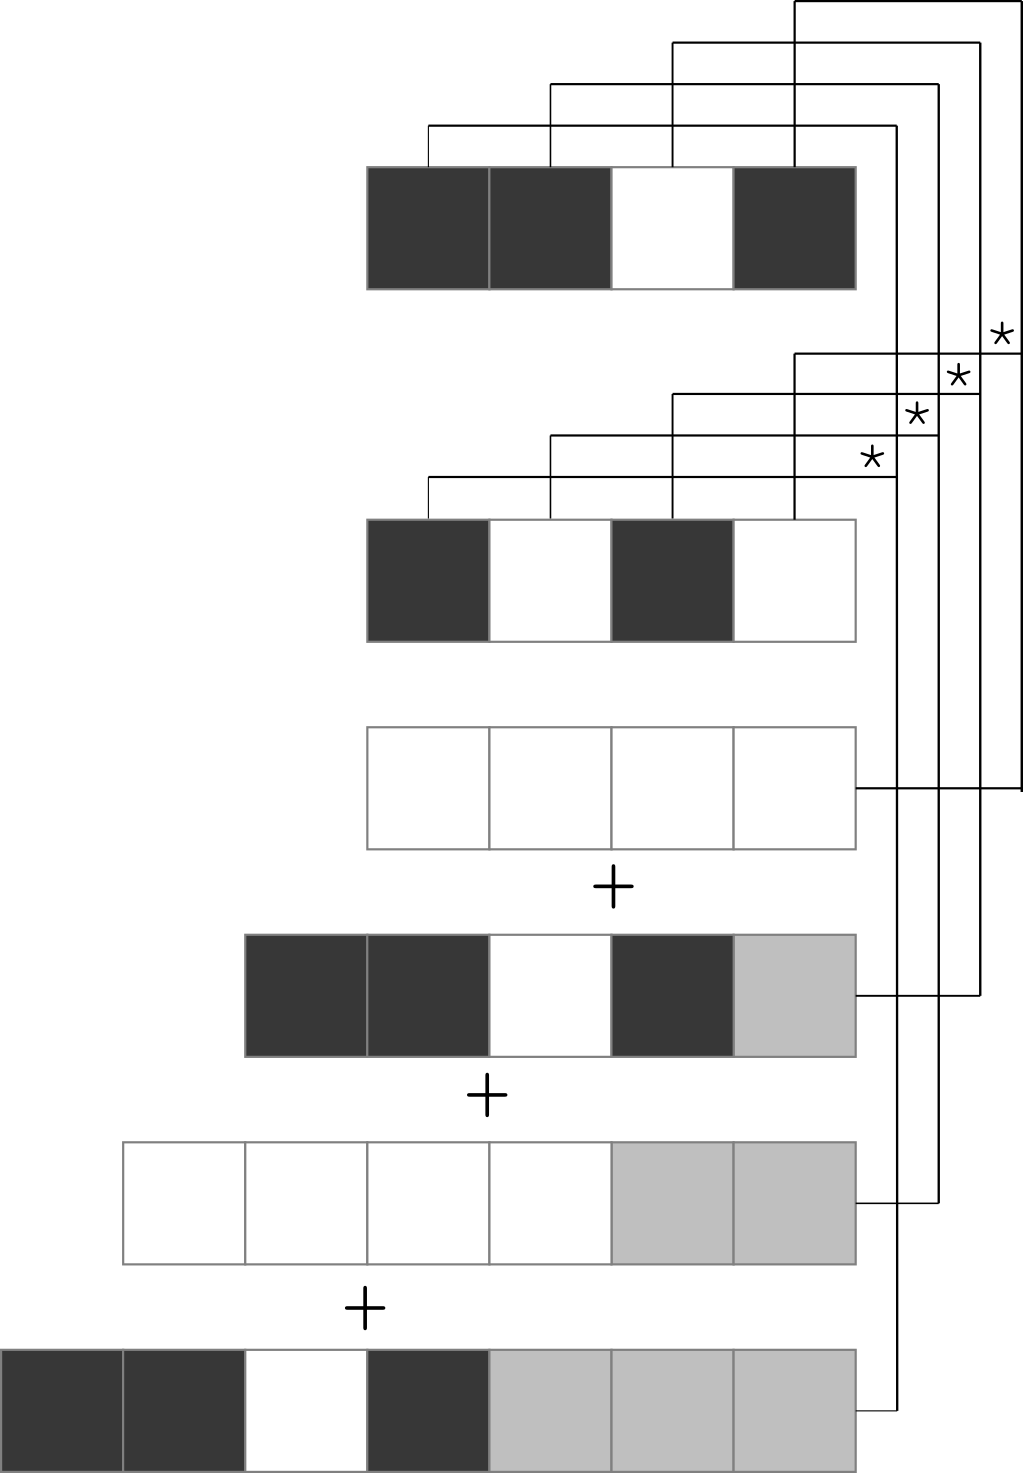
\includegraphics[width=\textwidth]{mult_float}
    \caption{Algoritmo de multiplicación}
    \label{fig:mult_float}
  \end{figure}

  \item \texttt{div}

  Operación de división (ver figura \ref{fig:div_float}). Es la operación más costosa porque requiere duplicar el tamaño (en bits) de los elementos, pero es esencial para realizar nuestro cálculo, y es el principal elemento que marca la diferencia con respecto al resto de implementaciones.

  \begin{lstlisting}[language=c++]
  void div_float(LweSample* result,
                  const LweSample* a, const LweSample* b,
                  const int float_bits, const int nb_bits,
                  const TFheGateBootstrappingCloudKeySet* bk);
  \end{lstlisting}

  %
  % void div(dividendo, b){
  %
  %   u_shiftl(divisor, b, nb_bits - 1, 2*nb_bits, bk);
  %
  %
  %
  %   for(int i = 0; i < nb_bits; i++) {
  %     // gt = dividendo >= divisor
  %     gte(gt, dividendo, divisor, 2*nb_bits, bk);
  %
  %     bootsCOPY(&cociente[nb_bits-i-1], &gt[0], bk);
  %
  %     // resto = gt? sub(dividendo, divisor) : resto
  %     sub(div_aux, dividendo, divisor, 2*nb_bits, bk);
  %     // divisor = shiftr(divisor, 1)
  %     u_shiftr(div_aux2, divisor, 1, 2*nb_bits, bk);
  %     for(int j = 0; j < 2*nb_bits; j++){
  %       bootsMUX(&resto[j], &gt[0], &div_aux[j], &dividendo[j], bk);
  %       // dividendo = gt ? resto : dividendo
  %       bootsMUX(&dividendo[j], &gt[0], &resto[j], &dividendo[j], bk);
  %       bootsCOPY(&divisor[j], &div_aux2[j], bk);
  %     }
  %   }
  % }
  %
  \begin{figure}[h]
    \centering
    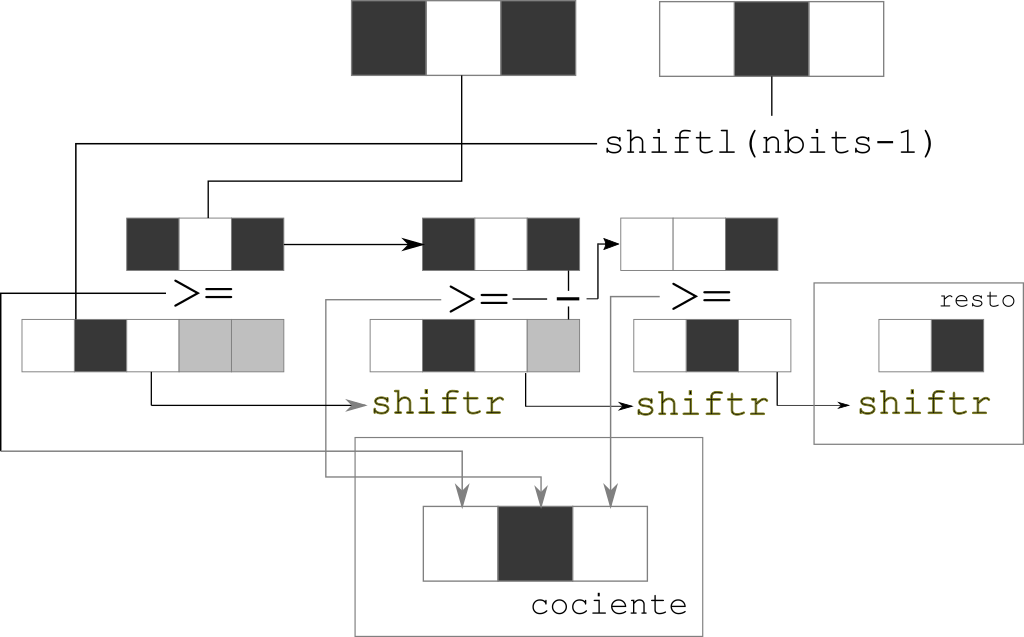
\includegraphics[width=\textwidth]{div_float}
    \caption{Algoritmo de división}
    \label{fig:div_float}
  \end{figure}


\end{itemize}

\section{Implementación con SEAL}

\subsection{Cálculo de la posición}

El sistema CKKS ofrece la posibilidad de trabajar con varios datos a la vez codificándolos como vectores. Hemos aprovechado esta característica para poder resolver la distancia entre el punto introducido por el usuario y las distintas curvas en una sola llamada, aplicando las operaciones necesarias en todas las curvas al mismo tiempo.

Procedemos de la siguiente manera:

\begin{enumerate}
    \item Generamos un vector $A$ con los valores $a$ de todas las curvas, otro $B$ con los valores $b$ y otro $C$ con los valores $c$ de las curvas.
    \item Codificamos todos estos vectores con \verb|CKKSEncoder|

    \item Determinamos el punto $y$ correspondiente al valor $x$ introducido por el usuario.
    Como sólo podemos hacer una operación en cada paso, tenemos que descomponer la sustitución en varias operaciones. En cada producto, al estar utilizando el esquema CKKS, tendremos que reescalar (y realinearizar, cuando los cálculos pendientes así lo requieran) nuestro resultado. La operación de reescalado trunca el número (le quita bits, ver \ref{tag:ckks}) y modifica los parámetros de cifrado reduciendo el número de operaciones restantes que podemos realizar con él. Por lo tanto, hay que intentar realizar el menor número de productos posible. Por ejemplo, si hubiese que hacer la operación $x_4=x^4$, sería preferible hacer $x_2 = x^2, x_4 = x_2^2$ (con sólo dos productos) que $x_4 = x * x * x * x$ (con cuatro).

    Además, al realizar el reescalado estamos obteniendo un número con una escala menor que el número que hemos cifrado inicialmente, por lo que cuando queramos sumar dos variables tenemos que asegurarnos de ajustarlas entre sí o saltará una excepción. Estas operaciones realmente se corresponden con eliminar valores de una cadena que gestiona \verb|SEALContext| en la que se especifican los parámetros de cifrado de cada fase.

    Tras realizar este estudio, procedemos a calcular:
    \begin{enumerate}
        \item $p_1 = x^2$
        \item Realinearización y reescalado de $p_1$. Aquí realinearizamos porque este elemento es el que más productos va a tener ($ A * x^2$ conlleva tres productos, mientras que $B * x$ sólo uno).
        \item $p_2 = p_1 * A$
        \item Reescalado de $p_2$
        \item $p_3 = B*x$
        \item Reescalado de $p_3$
        \item $p = p_2 + p_3$
        \item Doble reescalado de $C$ para poder sumarlo con $p$
        \item $y = p + C$
    \end{enumerate}

    \begin{gather}
        \begin{pmatrix}
            d_1 \\
            d_2 \\
            \vdots{} \\
            d_n
        \end{pmatrix}
        =
        \begin{pmatrix}
            y \\
            y \\
            \vdots{} \\
            y
        \end{pmatrix}
        - (x^2 *
        \begin{pmatrix}
            a_1 \\
            a_2 \\
            \vdots{} \\
            a_n
        \end{pmatrix}
        + x *
        \begin{pmatrix}
            b_1 \\
            b_2 \\
            \vdots{} \\
            b_n
        \end{pmatrix}
        +
        \begin{pmatrix}
            c_1 \\
            c_2 \\
            \vdots{} \\
            c_n
        \end{pmatrix}
        )
        \label{form:distancias_seal}
    \end{gather}

    \item Finalmente, como nuestro $y$ es el resultado de dos reescalados, tendremos que reescalar dos veces el $y$ introducido por el usuario (al que llamaremos $y_0$) para poder operar. Tras hacerlo, devolvemos el resultado \verb|encrypted_result| igual a $y - y_0$.

\end{enumerate}

Cuando el usuario descifre \verb|encrypted_result|, obtendrá un vector con las distancias entre el punto que ha introducido y todas las curvas, similar al de la figura \ref{form:distancias_seal}.

\section{Implementaciones Cliente/Servidor}

Finalmente, para cada una de las tecnologías se han desarrollado dos programas que hacen las funciones de cliente y servidor. De esta forma separamos la lógica de cifrado y descifrado (perteneciente a los clientes) y la lógica de procesado de los datos cifrados (propia de los servidores).

Para ambas, se ha programado una clase cliente, y una clase servidor, como hemos comentado cada una con las funciones que le son propias por su rol en la arquitectura, y para el desarrollo del trabajo hemos creado cuatro ejecutables que, apoyándose en las clases cliente/servidor implementarán la lógica para generar la curva de regresión y evaluar en el resultado los valores. De ahora en adelante cuando hablemos de cliente y servidor nos referiremos a estos ejecutables.

\subsubsection{TFHE}

El cliente TFHE ofrece la posibilidad de:

\begin{enumerate}
    \item Generar datos cifrados de la temperatura en Cabo de Gata guardando los $n$ valores de las $x$ con el formato \verb|ciudad_AXn.data| y los de las $y$ como  \verb|ciudad_AYn.data|).
    \item Generar datos cifrados de la temperatura en Finisterre siguiendo el mismo formato que anteriormente, pero con el prefijo \verb|ciudad_B|.
    \item Analizar los resultados generados por el servidor (indicándole la ruta en la que están, busca los archivos \verb|{a,b,c}.data|
    \item Descifrar un archivo cifrado con TFHE
\end{enumerate}{}

Cuando genera los datos cifrados, además exporta al sistema de archivos las claves para poder descifrar estos archivos cuando sea necesario, y poder subir la pública al servidor para procesar los datos.

El módulo que hace las veces de servidor con TFHE generará los parámetros $a$, $b$ y $c$ de los que llevamos hablando toda la sección en base a los archivos \verb|ciudad_...| que haya en la carpeta que se le indique. Como el proceso es muy lento, almacenará los resultados de las operaciones intermedias para recurrir a ellos si se corta la ejecución (ver figura \ref{fig:resultados_tfhe}), hasta generar los archivos $a.data$, $b.data$ y $c.data$.

\begin{listing}[ht]
    \begin{minted}{console}
    junquera@opa:~/UEM/TFM/results/tfhe/ciudad_A/resultados\$ ls -la
    total 4240
    drwxrwxr-x 2 junquera junquera   4096 ago 27 22:29 .
    drwxrwxr-x 3 junquera junquera   4096 ago 16 10:06 ..
    -rw-rw-r-- 1 junquera junquera 129024 ago 27 20:33 a.data
    -rw-rw-r-- 1 junquera junquera 129024 ago 27 08:22 b.data
    -rw-rw-r-- 1 junquera junquera 129024 ago 25 23:22 c.data
    -rw-r--r-- 1 junquera junquera 129024 ago 16 10:06 i2.data
    -rw-rw-r-- 1 junquera junquera 129024 ago 24 07:08 i2l2.data
    ...
    -rw-rw-r-- 1 junquera junquera 129024 ago 23 20:06 ul.data
    -rw-rw-r-- 1 junquera junquera 129024 ago 16 10:06 v.data
    -rw-rw-r-- 1 junquera junquera 129024 ago 23 20:06 vl.data
    -rw-rw-r-- 1 junquera junquera 129024 ago 16 10:06 w.data
    -rw-rw-r-- 1 junquera junquera 129024 ago 23 20:06 wj.data
    \end{minted}
    \caption{Archivos generados por el servidor TFHE} \label{fig:resultados_tfhe}
\end{listing}

Para hacer una prueba lo más realista posible de todo el sistema, he cifrado los datos que he obtenido de AEMET (ver anexo \ref{appendix:datos_aemet}) de las temperaturas en las dos ciudades con el cliente de TFHE, y los he subido a la nube de Digital Ocean (\url{https://www.digitalocean.com/}) para procesarlos con el código del servidor TFHE.

Tras finalizar el cálculo, los he descargado y descifrado con el cliente TFHE, y he insertado manualmente los resultados (ver tabla \ref{table:r2_cg_ft}) en el código del servidor SEAL.

\begin{table}[]
    \centering
    \begin{tabular}{c c c c}
        Ubicación  & a & b & c \\
        \hline \hline 
        Cabo de Gata    & $-0.413$ & $5.928$ & $2.423$ \\
        Finisterre    & $-0.261$ & $3.801$ & $5.041$
    \end{tabular}
    \caption{Resultados del servidor TFHE}
    \label{table:r2_cg_ft}
\end{table}

El código fuente se encuentra disponible en \url{https://gitlab.com/junquera/tfhe-cs}.

\subsubsection{SEAL}


El servidor (\verb|server.main|) lee de la carpeta en la que se está ejecutando los archivos cifrados \verb|x.data| y \verb|y.data| generados por el cliente, y los elementos criptográficos necesarios (clave pública, clave de realinearización y parámetros de cifrado). Tras procesar estos datos con los valores de las curvas que ha calculado previamente en TFHE, genera el archivo \verb|result.data| y un archivo de texto con los nombres de las curvas (para que el cliente pueda interpretar los resultados).

El \verb|main| del cliente (codificado en el archivo \verb|client-main.cpp|) tiene dos funcionalidades:
\begin{enumerate}
    \item En la primera pide que se introduzcan dos valores (temperatura y fecha), los cifra y genera dos archivos: \verb|x.data| y \verb|y.data|.

    \item La otra funcionalidad, que se ejecuta tras la ejecución del código del servidor lee el archivo  \verb|result.data| de la carpeta en la que se ejecuta, lo descifra e imprime por pantalla el resultado combinado del vector descifrado con el archivo \verb|curve_names.data|. En \ref{fig:ejecuta_seal_cs} se puede ver la ejecución del sistema completo.

  \begin{figure}[h]
    \centering
    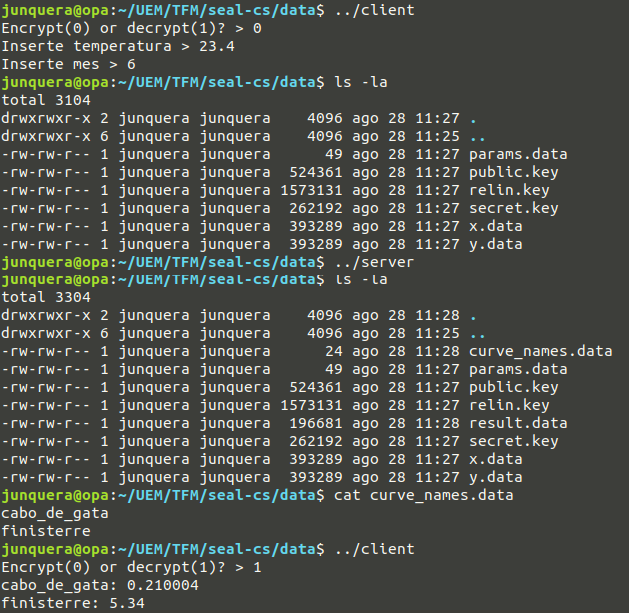
\includegraphics[width=0.75\textwidth]{ejecuta_seal_cs}
    \caption{Ejecución completa del sistema de SEAL} \label{fig:ejecuta_seal_cs}
  \end{figure}
\end{enumerate}

El código fuente se encuentra disponible en \url{https://gitlab.com/junquera/seal-cs}. Para más información consultar el apéndice \ref{appendix:manual}.

\section{Evaluación de límites y rendimientos}

Por último se han desarrollado varios archivos de prueba para evaluar los límites y el rendimiento de las librerías. Estas pruebas son la culminación de este estudio, y buscan aportar un enfoque cuantitativo a su funcionamiento, más allá de los cálculos que se puedan hacer con el conocimiento de las tecnologías o la visión empírica desde el punto de vista del desarrollador.


\subsubsection{TFHE}

Para evaluar la eficiencia de TFHE ejecutamos todas las funciones aritméticas que hemos escrito en \verb|tfhe-math| con distintos tamaños de texto cifrado (desde 4 hasta 64 bits) calculando el tiempo que tardan en realizarse. En el capítulo de resultados (capítulo \ref{chap:resultados}) veremos la comparativa entre los resultados obtenidos y el tiempo estimado en base a la teoría.

\subsubsection{SEAL}

Con SEAL hemos desarrollado dos tipos de pruebas:

\begin{itemize}
    \item Al igual que con TFHE, hemos evaluado el tiempo que tarda en realizar las operaciones aritméticas (en este caso, sólo suma y multiplicación) con distintos tamaños de texto cifrado.
    \item También hemos evaluado cuáles son los límites de cómputo con distintos tamaños de texto cifrado, con y sin aplicar realinearizaciones.
\end{itemize}

Además entre los códigos de ejemplo de SEAL se encuentra un programa para evaluar la eficiencia de sus esquemas. Lo incluiremos entre nuestras pruebas.

Ya sólo queda analizar los resultados de todos nuestros experimentos.

\chapter{Resultados}
\label{chap:resultados}

\section{TFHE}

Al ser una ejecución "especulativa"...

\subsection{Tiempos de ejecución}

\subsection{Tamaño máximo de los datos}

% log(X, 2)*max_exponente <= (64 bits de entero - 10 bits de decimal - 1 bit de signo) = 53 bits

% 4 < max_exponente < 10

% X < 32

\subsection{Problemas encontrados}

- Signo

- Floats

- Eficiencia

% TODO Documentar tiempos

- Tamaño de los datos al multiplicar...

% TODO Mostrar algunos ejemplos de codificación de números en bits
l = sum(1, n)
nb_bits > 1 + math.log(n, 2) + 10

\section{Coste de la implantación}

Equipo de ingenieros, estudio, pruebas...

Máquina digital ocean con cálculo (tiempo*precio).

Los resultados para curva A han sido: ...
para curva B han sido: ...

\section{SEAL}

\subsection{Tiempos de ejecución}

\subsection{Límites de cómputo}

Con CKKS, por tamaño de la cadena:

El primer y el último número de la cadena tienen que ser mayores que el número a cifrar/descifrar, y los intermedios tienen que ser lo algo más grandes  que los intermedios para asegurar la precisión, y la suma de estos dos con los intermedios tiene que ser menos que  \verb|max coeff_modulus| bit-length. POr lo tanto:

\begin{itemize}
    \item Para un número de 40 bits, es necesario utilizr al menos  \verb|poly_modulus_degree de 8192|, y se pueden hacer 4 operaciones.
    \item Para un número de 64 bits, es necesario utilizr al menos  \verb|poly_modulus_degree de 16384|, y se pueden hacer 7 operaciones.
    \item Para un número de 64 bits, es necesario utilizr al menos \verb|poly_modulus_degree de 16384|, y se pueden hacer 14 operaciones.
\end{itemize}

Este es el número de operaciones tras el cual el resultado es inválido.

\begin{lstlisting}
+----------------------------------------------------+
| poly_modulus_degree | max coeff_modulus bit-length |
+---------------------+------------------------------+
| 1024                | 27                           |
| 2048                | 54                           |
| 4096                | 109                          |
| 8192                | 218                          |
| 16384               | 438                          |
| 32768               | 881                          |
+---------------------+------------------------------+
\end{lstlisting}

Con BFV sólo enteros, y por niveles de error:

\chapter{Conclusiones}
\label{chap:conclusiones}

- Ya no es solo la eficiencia, es muy dificil programar

- Hay que saber mucho para hacerlo, y más para hacerlo correctamente (\cite{peng_danger_2019})

- Como hemos visto, la seguridad tiene que implementarse en función del riesgo. Estas implementaciones pueden ser útiles para operaciones comunes, por ejemplo, en nubes públicas, siempre que el valor del activo así lo requiera.

- Reto de TFHE: http://lab.algonics.net/slides_ac16/index-asiacrypt.html#/38

\chapter{Trabajos futuros}

- Estudio del nuevo estándar 4

\part*{Apéndices}
\label{chap:apendices}

%Apéndices

% Bibliografía

% (SEGUIR NORMA APA)

% Apellido1, N., & Apellido2, N. (2002). Título. Editorial.
% Autor. (2018). Título. Obtenido de Título sitio web: https://url.com/url.pdf
% Título. (03 de 11 de 2006). Obtenido de https://www.url.com/url.pdf


% Diario de Experimentos

% Manual de Instalación

% Manual de Usuario

% Guía de solucionado de errores


\bibliographystyle{apa}
\nocite{*}
\bibliography{references.bib}
% \input{bib}
% \input{experimentos}
% \input{manual_instalacion}
% \input{manual_usuario}

\end{document}
